% =============================================================================
%  The assumptions of a one-dimensional PBL closure, as a pyramid -- VARIANT: scale separation split into its two
%  conditions (spectral gap at the left, gradient scale at the right), so that the K-form stands on Rotta, the eddy
%  viscosity and locality. Derived from pbl_assumptions_pyramid.tex on 2026-09-17; its vertical twin is
%  pbl_assumptions_pyramid_split_vertical.tex (python3 scripts/make_pyramid_vertical.py pbl_assumptions_pyramid_split.tex).
%  2026-09-17: ONLY THE VERTICAL TWIN IS MAINTAINED (Elias). Block extents along the ground are sized for the vertical
%  page (extent x 0.86 = block height there); built directly, this landscape page has overflowing texts.
%  Shift coordinates with scripts/pyramid_remap.py, never by hand.
%  Companion to pbl_assumptions_table.tex (rows A1-C10 = Table I.1; D3-D8 added here).
%  Build: source ~/miniconda3/bin/activate tex && tectonic pbl_assumptions_pyramid.tex
%  Layout rule: a block touches at its bottom exactly the blocks it relies on; blocks
%  on one level never touch (air gap 0.10 cm). Three tiers (2026-09-16, third version):
%  premises = physical hypotheses (dark grey) / concepts of turbulence theory (light grey) /
%  formal statements of the level-2.5 closure (white). No row abbreviations on the
%  blocks; the mapping to the note's rows is in the last paragraph. Unit width 1.15 cm,
%  doubles 2.40, triples 3.65; tier 1 starts at x = 0.6; tier labels at x = -0.3.
%  Ground order forced by the adjacency chain SEP-MIX-HOM-STA-SIM-ISOb-AXI-BOU (mixing split off
%  scale separation 2026-09-16 evening: ergodicity in space rests on mixing + homogeneity).
%  Frames (\hl): purple = 3D closure, red = Goger 2019, nested = both (decisive cells of Table I.0).
%  Re-added after the audit (Elias 2026-09-16): B5 energy lost, B4 not advected, C6 vertical Ri,
%  C8 no redistribution, C4 blind to terrain and grid. Left in the note only: C2's Pr(Ri), third moments.
% =============================================================================
\documentclass[10pt]{article}
\usepackage{iftex}
\ifPDFTeX
  \usepackage[utf8]{inputenc}
  \usepackage[T1]{fontenc}
  \usepackage{lmodern}
\else
  \usepackage{fontspec}
  \setmainfont{lmroman10-regular.otf}[BoldFont=lmroman10-bold.otf,
    ItalicFont=lmroman10-italic.otf, BoldItalicFont=lmroman10-bolditalic.otf]
\fi
\usepackage[british]{babel}
\usepackage[a4paper,landscape,margin=10mm,top=7mm,bottom=7mm]{geometry}
\usepackage{amsmath,amssymb}
\usepackage{xcolor}
\usepackage{tikz}
\usepackage{microtype}
\pagestyle{empty}
\setlength{\parindent}{0pt}
\setlength{\parskip}{0.5ex}
% rigid math relation spacing: the centred block texts would otherwise stretch around = and <<
\thickmuskip=5mu \medmuskip=4mu \thinmuskip=3mu

% ---- notation ---------------------------------------------------------------
\newcommand{\avg}[1]{\langle #1 \rangle}
\newcommand{\pd}[2]{\partial #1/\partial #2}
\newcommand{\qsq}{q^{2}}
\newcommand{\Rfc}{R_{fc}}
\newcommand{\dx}{\Delta x}
% ---- rows the PhD concept turns on (same data as the note's macros.tex) ------
\definecolor{cKey}{HTML}{7B2D8E}
\definecolor{cGXIX}{HTML}{990011}   % Goger 2019 port (the note's colour)
\definecolor{cFULL}{HTML}{7B2D8E}   % Kosovic-Juliano 3D closure (the note's colour)
% \hl{x0}{x1}{y0}{y1}{colour}{inset}: a frame inside a block, marking a scheme's decisive block
\newcommand{\hl}[6]{\draw[#5, line width=1.1pt] (#1+#6,#3+#6) rectangle (#2-#6,#4-#6);}
\newcommand{\setkey}[2]{\expandafter\def\csname key@#1\endcsname{#2}}
\makeatletter
\setkey{A1}{1}\setkey{B1}{1}\setkey{B2}{1}\setkey{B3}{1}\setkey{C3}{1}\setkey{C4}{1}\setkey{C6}{1}\setkey{C7}{1}
\setkey{B5}{2}\setkey{B6}{2}\setkey{C2}{2}\setkey{C5}{2}\setkey{C9}{2}
\newcommand{\keymark}[1]{\ifcsname key@#1\endcsname
  \if1\csname key@#1\endcsname\textcolor{cKey}{$\blacktriangleright$}\else\textcolor{cKey}{$\triangleright$}\fi\fi}
\makeatother
\newcommand{\pid}[1]{\keymark{#1}\textbf{#1}}
% \pb{x0}{x1}{y0}{y1}{style}{text}: a block from (x0,y0) to (x1,y1), text centred
\newcommand{\pbf}[7]{\pgfmathsetmacro{\pbw}{#2-#1-#7}%
  \draw[#5] (#1,#3) rectangle (#2,#4);
  \node[align=center, font=\tiny, inner sep=0pt, text width=\pbw cm] at ({(#1+#2)/2},{(#3+#4)/2}) {#6};}
% \pbunion{style}{tx}{ty}{tw}{text}{pieces x0/x1/y0/y1,...}{outline (x,y) -- ...}: one block of several rectangles
\newcommand{\pbunion}[7]{\foreach \ux/\uX/\uy/\uY in {#6} {\fill[black!22] (\ux,\uy) rectangle (\uX,\uY);}
  \draw[#1, fill=none] #7 -- cycle;
  \node[align=center, font=\tiny, inner sep=0pt, text width=#4 cm] at (#2,#3) {#5};}
\newcommand{\pb}[6]{\pgfmathsetmacro{\pbw}{#2-#1-0.20}%
  \draw[#5] (#1,#3) rectangle (#2,#4);
  \node[align=center, font=\tiny, inner sep=0pt, text width=\pbw cm] at ({(#1+#2)/2},{(#3+#4)/2}) {#6};}


% ---- the hectometre-scale column (used by the VERTICAL version only; read by scripts/make_pyramid_vertical.py)
% \hecto{<formal statement title>}{<what becomes of it at Delta = 500 m over the Inn Valley>}; no-op here.
% Sources: the mountain and grey-zone columns of the note's Table I.1 and the project's own runs.
\newcommand{\hecto}[2]{}
\hecto{Grid means are ensemble means}{By day much of the kinetic energy at the lowest levels is resolved, the effective resolution is several $\Delta$, and the partition claim waits for a $w$-spectrum below that scale; the resolved shear then enters production twice. At night the eddies shrink far below $\Delta$: the cell holds only a few integral scales and the vertical grid none, the cell statistic is a single realisation, and the stable regime is mesoscale again. On a slope the cell mixes slope layer and valley core.}
\hecto{Vertical shear only}{The jet's cross-valley shear is a sizeable fraction of its vertical shear; in weak drainage flow directional shear sets $u_*$.}
\hecto{Vertical divergence only}{Horizontal flux divergences are of the order of the vertical one, and the Riviera budgets closed only with transport and advection; the numerical operator stands where the physical divergence belongs, and the energy it removes vanishes instead of feeding $\qsq$.}
\hecto{Wall value of $\qsq$}{The nocturnal sonics record turbulence at the surface where every model goes laminar; the observed friction velocity implies a wall $\qsq$ between the two closures' values.}
\hecto{Level-2.5 truncation}{Transitions outrun $l/q$; the strain cap's footprint measures it.}
\hecto{Stability functions and cutoff}{Most nocturnal valley cells lie beyond the critical Richardson number, where the deficit against the control is flat; the approximate closure switches off at $\Rfc$, the others never.}
\hecto{Surface fluxes and first level}{The katabatic jet maximum sits inside the layer; over forest the first level lies in the roughness sublayer; the momentum flux is rarely height-constant.}
\hecto{Master length scale}{$z_i$ is ill-posed under elevated inversions, the wall distance ambiguous on a slope, the horizontal eddy set by the valley width: two lengths. In the cold pool the length, not the fluxes, was the lever; the fork bounds it by a buoyancy limit and a strain cap.}
\hecto{Constant set}{Three constant sets in one comparison; their dissipation constants differ by a factor that rivals the effects to be reported.}
\hecto{One length for $K$ and $\varepsilon$}{$\varepsilon$ is filter-independent while $q^3$ is not, so the dissipation length must shrink with the grid; the inertial-subrange estimate from the sonics needs Taylor's hypothesis and fails in weak-wind nights.}
\hecto{Pressure terms}{Taking them small is ``a dangerous assumption'' in complex terrain; the Radfeld budget residual is their only observation.}
\hecto{K-form fluxes}{By day the eddies span $z_i$ and heat runs against the local gradient: the plume terms exist for this. Where slope wind turns into valley wind the stress axes leave the gradient and the jet veers with height: $\avg{uv}$ appears, negative production is admissible. The grid filter, aspect ratio 25, imprints its anisotropy on the subgrid eddies; in stable air $K_H/K_M$ falls with Ri.}
\hecto{Buoyancy term}{The slope-normal surface heat flux has a horizontal component with no home in the budget; in stable air buoyancy damps $\avg{w^2}$ selectively; on fog nights the saturated flux follows the moist gradient, which only the control's condensation scheme knows; $\beta = 1/300$~K is a few percent off at valley $\Theta_v$.}

% ---- dependencies the contact rule cannot draw (post-audit list; used by scripts/make_pyramid_graph.py). No-op here.
\newcommand{\lean}[2]{}
\lean{Boundary-layer (column) approximation}{Boussinesq}
\lean{Energy cascade}{Stationarity}
\lean{Local equilibrium}{Locality}
\lean{Local equilibrium}{Horizontal homogeneity}
\lean{Monin--Obukhov similarity}{Constant-flux layer}
\lean{Mixing length}{Mixing}
\lean{Locality}{Mixing}
\lean{Energy cascade}{Mixing}
\lean{Eddy viscosity}{Locality}
\lean{Eddy viscosity}{Mixing length}
\lean{Return to isotropy}{Horizontal homogeneity}
\lean{Stability functions and cutoff}{Level-2.5 truncation}
\lean{Universal constants}{Reynolds averaging}
\lean{Vertical divergence only}{Spectral gap}
\lean{Wall value of $\qsq$}{Universal constants}
\lean{Stability functions and cutoff}{Universal constants}
\lean{Stability functions and cutoff}{Boundary-layer (column) approximation}
\lean{Stability functions and cutoff}{Buoyancy production}
\lean{Stability functions and cutoff}{Local equilibrium}
\lean{Master length scale}{Buoyancy term}
\lean{Buoyancy term}{K-form fluxes}
\lean{Pressure terms}{Locality}
\lean{Pressure terms}{Universal constants}
\lean{One length for $K$ and $\varepsilon$}{Master length scale}
\lean{K-form fluxes}{Master length scale}
\lean{K-form fluxes}{Stability functions and cutoff}
% ---- scheme quicklook (moons above the formalism tier; scripts/make_moons.py rewrites the strip)
% \moon{<block title>}{K|P|D x4} in the order MYNN as run, G19 port, 3D-APPROX, 3D-FULL; from Table I.0 of the note:
% a block is K if all its rows are kept, D if all are dropped, else P. No-op here (data only).
\newcommand{\moon}[2]{}
\moon{Grid means are ensemble means}{P K P P}
\moon{Vertical shear only}{K P K D}
\moon{Vertical divergence only}{K P P D}
\moon{Wall value of $\qsq$}{K K D D}
\moon{Level-2.5 truncation}{K K K K}
\moon{Stability functions and cutoff}{D P K P}
\moon{Surface fluxes and first level}{K K K K}
\moon{Master length scale}{K P K K}
\moon{Constant set}{K K K K}
\moon{One length for $K$ and $\varepsilon$}{K K K K}
\moon{Pressure terms}{K K K K}
\moon{K-form fluxes}{P P P D}
\moon{Buoyancy term}{P P P P}
% glyphs (the note's), absolute size, colour = scheme identity
\newcommand{\gK}{\tikz[baseline=-0.6ex]{\fill (0,0) circle (0.11);}}
\newcommand{\gP}{\tikz[baseline=-0.6ex]{\draw[line width=0.5pt] (0,0) circle (0.11); \fill (0,0) -- (90:0.11) arc (90:270:0.11) -- cycle;}}
\newcommand{\gD}{\tikz[baseline=-0.6ex]{\draw[line width=0.5pt] (0,0) circle (0.11);}}
\definecolor{cMYNN}{HTML}{3A6B00}    % MYNN as run
\definecolor{cAPPROX}{HTML}{9A5AA8}  % 3D-APPROX

\begin{document}
{\Large\bfseries The assumptions of a one-dimensional PBL closure, as a pyramid: what rests on what}\\[0.3ex]
{\small Companion to the assumptions note; three tiers. Variant of 2026-09-17: scale separation split into its two conditions, and the closure's $K = lqS$ kept apart from the K-form.}

\vspace{0.6ex}
{\footnotesize Every block is an assumption a boundary-layer scheme makes in order to run. A block touches at its
bottom exactly the blocks it relies on, and blocks on one level do not touch each other. Three tiers. Dark grey, the ground: nine hypotheses about the fluid and the flow that rest on nothing else here; horizontal homogeneity extends under stationarity and rises between stationarity and similarity, with an air gap above the tunnel, so that Monin--Obukhov similarity touches its three premises. Light grey, the
concepts: the constructs of turbulence theory that follow from the ground and that every closure of this family
speaks in --- Reynolds averaging, the column approximation, the constant-flux layer, Monin--Obukhov similarity,
the mixing length, the eddy viscosity, Rotta's return to isotropy, Kolmogorov's cascade. White, the formalism:
the statements of the level-2.5 closure as written, each resting on the concepts it applies. Each block shows its
primary reliance; the incidence matrix of the note has the full set. Where a block leans on a parent it cannot touch, its own text names that parent, as in ``$W = 0$ by continuity''; the two premises without a block, high Reynolds number and unsaturated air, are named in the premise they qualify. Not drawn, because no scheme needs them to
run: ergodicity in time and Taylor's hypothesis, which carry the observations and the calibration; the
constraints realizability and Galilean invariance, which bound the algebra rather than carry a block; and the
dynamical core's numerical dissipation. Homogeneity carries a channel: it runs through stationarity and similarity and surfaces as a band on the contact edge, where Monin--Obukhov similarity and the mixing length touch it. Scale separation appears as its two conditions, the spectral gap at the left under the averaging and the gradient scale at the right under gradient transport. The K-form stands on locality and the eddy viscosity alone, and the eddy viscosity on the gradient scale and the axisymmetry of the mixing; how this closure builds its $K = lqS$ is not part of the K-form: $l$ is the master length, $S$ the stability functions, which stand on Rotta's return, and $q$ the prognostic energy. Strict horizontal homogeneity already makes the surface horizontal, so the axisymmetry premise keeps only what homogeneity does not give: one $K$ along and across the shear. The moons above the formalism tier are the quicklook on the four schemes of the concept's first research question, rows from bottom to top \textcolor{cMYNN}{\textbf{MYNN as run}}, \textcolor{cGXIX}{\textbf{G19 port}}, \textcolor{cAPPROX}{\textbf{3D-APPROX}}, \textcolor{cFULL}{\textbf{3D-FULL}}: \gK{} the scheme as run implements the assumption, \gP{} partly, \gD{} drops it; a block takes the status of its rows in the note's Table~I.0, kept only when all are kept, dropped only when all are dropped.\par}

\vspace{0.4ex}
\begin{center}
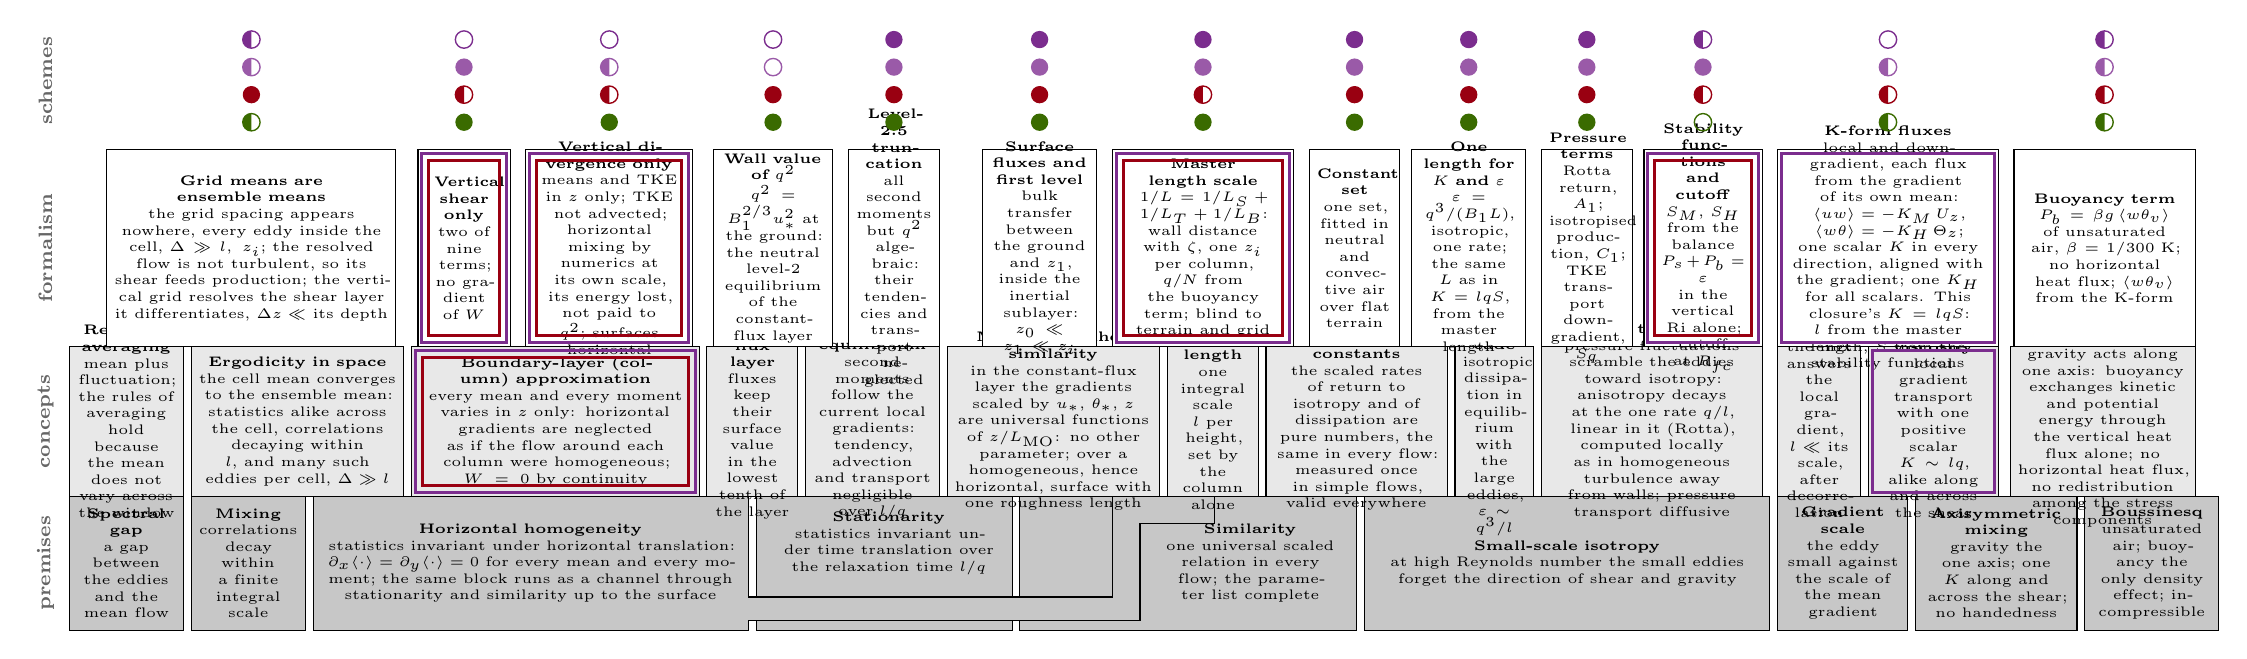
\begin{tikzpicture}[x=1cm, y=1cm,
  ground/.style={draw, line width=0.4pt, fill=black!22},
  hyp/.style={draw, line width=0.4pt, fill=black!9},
  row/.style={draw, line width=0.4pt, fill=white},
  tier/.style={font=\scriptsize\bfseries, rotate=90, anchor=center, text=black!60}]
% ---- tier labels -----------------------------------------------------------------------------------
\node[tier] at (-0.3, 0.85) {premises};
\node[tier] at (-0.3, 2.65) {concepts};
\node[tier] at (-0.3, 4.85) {formalism};
% ---- tier 0: physical hypotheses (y 0 -- 1.7); each boundary sits under the concept that spans it --
\pb{0}{1.45}{0}{1.7}{ground}{\textbf{Spectral gap}\\ a gap between the eddies and the mean flow}
\pb{1.55}{3}{0}{1.7}{ground}{\textbf{Mixing}\\ correlations decay within a finite integral scale}
% order forced by the adjacency chain SEP-MIX-HOM-STA-SIM-ISOb-AXI-BOU (unit 1.15, gap 0.10, offset 0.6);

% mixing is one block: body + a channel through the bottom of scale separation that surfaces as a band under locality's left part

\pbunion{ground}{10.41}{1.1}{3.3}{\textbf{Stationarity}\\ statistics invariant under time translation over the relaxation time $l/q$}{8.725/11.975/0.5/1.7,8.725/11.975/0/0.5}{(8.725,0) -- (8.725,1.7) -- (11.975,1.7) -- (11.975,0)}
\pbunion{ground}{15}{0.85}{2.5}{\textbf{Similarity}\\ one universal scaled relation in every flow; the parameter list complete}{13.7/16.35/0/1.7,12.075/13.7/0/1.7}{(12.075,0) -- (12.075,1.7) -- (16.35,1.7) -- (16.35,0)}
% homogeneity is one block: body + a channel through stationarity and similarity that surfaces as a band under Monin-Obukhov and the mixing length; drawn after them so it lies on top
\pbunion{ground}{5.86}{0.85}{5.3}{\textbf{Horizontal homogeneity}\\ statistics invariant under horizontal translation: \mbox{$\partial_x\avg{\cdot} = \partial_y\avg{\cdot} = 0$} for every mean and every moment; the same block runs as a channel through stationarity and similarity up to the surface}{3.1/8.625/0/1.7,8.625/13.6/0.12/0.42,13.25/13.6/0.12/1.7,13.25/14.55/1.35/1.7}{(3.1,0) -- (3.1,1.7) -- (8.625,1.7) -- (8.625,0.42) -- (13.25,0.42) -- (13.25,1.7) -- (14.55,1.7) -- (14.55,1.35) -- (13.6,1.35) -- (13.6,0.12) -- (8.625,0.12) -- (8.625,0)}
\pb{16.45}{21.6}{0}{1.7}{ground}{\textbf{Small-scale isotropy}\\ at high Reynolds number the small eddies forget the direction of shear and gravity}
\pb{21.7}{23.35}{0}{1.7}{ground}{\textbf{Gradient scale}\\ the eddy small against the scale of the mean gradient}
\pb{23.45}{25.5}{0}{1.7}{ground}{\textbf{Axisymmetric mixing}\\ gravity the one axis; one $K$ along and across the shear; no handedness}
\pb{25.6}{27.3}{0}{1.7}{ground}{\textbf{Boussinesq}\\ unsaturated air; buoyancy the only density effect; incompressible}


% ---- tier 1: concepts (y 1.7 -- 3.6); 7 singles of 1.15, 4 doubles of 2.40, 2 triples of 3.65 ------

\pb{0}{1.45}{1.7}{3.6}{hyp}{\textbf{Reynolds averaging}\\ mean plus fluctuation; the rules of averaging hold because the mean does not vary across the window}
\pb{1.55}{4.25}{1.7}{3.6}{hyp}{\textbf{Ergodicity in space}\\ the cell mean converges to the ensemble mean: statistics alike across the cell, correlations decaying within $l$, and many such eddies per cell, \mbox{$\Delta \gg l$}}
\pbf{4.35}{8}{1.7}{3.6}{hyp}{\textbf{Boundary-layer (column) approximation}\\ every mean and every moment varies in $z$ only: horizontal gradients are neglected as if the flow around each column were homogeneous; $W = 0$ by continuity}{0.44}
\pb{8.1}{9.25}{1.7}{3.6}{hyp}{\textbf{Constant-flux layer}\\ fluxes keep their surface value in the lowest tenth of the layer}
\pb{9.35}{11.05}{1.7}{3.6}{hyp}{\textbf{Local equilibrium}\\ second moments follow the current local gradients: tendency, advection and transport negligible over $l/q$}
\pb{11.15}{13.85}{1.7}{3.6}{hyp}{\textbf{Monin--Obukhov similarity}\\ in the constant-flux layer the gradients scaled by $u_*$, $\theta_*$, $z$ are universal functions of $z/L_{\mathrm{MO}}$: no other parameter; over a homogeneous, hence horizontal, surface with one roughness length}
\pb{13.95}{15.1}{1.7}{3.6}{hyp}{\textbf{Mixing length}\\ one integral scale $l$ per height, set by the column alone}
\pb{15.2}{17.5}{1.7}{3.6}{hyp}{\textbf{Universal constants}\\ the scaled rates of return to isotropy and of dissipation are pure numbers, the same in every flow: measured once in simple flows, valid everywhere}
\pb{17.6}{18.6}{1.7}{3.6}{hyp}{\textbf{Energy cascade}\\ isotropic dissipation in equilibrium with the large eddies, $\varepsilon \sim q^3/l$}
\pb{18.7}{21.5}{1.7}{3.6}{hyp}{\textbf{Return to isotropy}\\ pressure fluctuations scramble the eddies toward isotropy: anisotropy decays at the one rate $q/l$, linear in it (Rotta), computed locally as in homogeneous turbulence away from walls; pressure transport diffusive}
\pbf{22.85}{24.5}{1.7}{3.6}{hyp}{\textbf{Eddy viscosity}\\ local gradient transport with one positive scalar $K \sim l q$, alike along and across the shear}{0.30}
\pb{21.7}{22.75}{1.7}{3.6}{hyp}{\textbf{Locality}\\ the flux answers the local gradient, $l \ll$ its scale, after decorrelation}

\pb{24.65}{27}{1.7}{3.6}{hyp}{\textbf{Buoyancy production}\\ gravity acts along one axis: buoyancy exchanges kinetic and potential energy through the vertical heat flux alone; no horizontal heat flux, no redistribution among the stress components}
% ---- tier 2: the formalism (y 3.6 -- 6.1) --------------------------------------------------------------

\pb{0.48}{4.15}{3.6}{6.1}{row}{\textbf{Grid means are ensemble means}\\ the grid spacing appears nowhere, every eddy inside the cell, $\Delta \gg l,\ z_i$; the resolved flow is not turbulent, so its shear feeds production; the vertical grid resolves the shear layer it differentiates, $\Delta z \ll$ its depth}
\pbf{4.43}{5.6}{3.6}{6.1}{row}{\textbf{Vertical shear only}\\ two of nine terms; no gradient of $W$}{0.44}
\pbf{5.8}{7.92}{3.6}{6.1}{row}{\textbf{Vertical divergence only}\\ means and TKE in $z$ only; TKE not advected; horizontal mixing by numerics at its own scale, its energy lost, not paid to $\qsq$; surfaces horizontal}{0.36}
\pb{8.18}{9.7}{3.6}{6.1}{row}{\textbf{Wall value of $\qsq$}\\ $\qsq = B_1^{2/3} u_*^2$ at the ground: the neutral level-2 equilibrium of the constant-flux layer}
\pb{9.9}{11.05}{3.6}{6.1}{row}{\textbf{Level-2.5 truncation}\\ all second moments but $\qsq$ algebraic: their tendencies and transport neglected}
\pb{11.6}{13.05}{3.6}{6.1}{row}{\textbf{Surface fluxes and first level}\\ bulk transfer between the ground and $z_1$, inside the inertial sublayer: $z_0 \ll z_1 \ll z_i$}
\pbf{13.25}{15.55}{3.6}{6.1}{row}{\textbf{Master length scale}\\ $1/L = 1/L_S + 1/L_T + 1/L_B$: wall distance with $\zeta$, one $z_i$ per column, $q/N$ from the buoyancy term; blind to terrain and grid}{0.44}
\pb{15.75}{16.9}{3.6}{6.1}{row}{\textbf{Constant set}\\ one set, fitted in neutral and convective air over flat terrain}
\pb{17.05}{18.5}{3.6}{6.1}{row}{\textbf{One length for $K$ and $\varepsilon$}\\ $\varepsilon = q^3/(B_1 L)$, isotropic, one rate; the same $L$ as in $K = lqS$, from the master length}
\pb{18.7}{19.85}{3.6}{6.1}{row}{\textbf{Pressure terms}\\ Rotta return, $A_1$; isotropised production, $C_1$; TKE transport down-gradient, $S_q$}
\pbf{20}{21.5}{3.6}{6.1}{row}{\textbf{Stability functions and cutoff}\\ $S_M$, $S_H$ from the balance $P_s + P_b = \varepsilon$\\ in the vertical Ri alone; cutoff at $\Rfc$}{0.44}
\pbf{21.7}{24.5}{3.6}{6.1}{row}{\textbf{K-form fluxes}\\ local and down-gradient, each flux from the gradient of its own mean: \mbox{$\avg{uw} = -K_M\,U_z$}, \mbox{$\avg{w\theta} = -K_H\,\Theta_z$}; one scalar $K$ in every direction, aligned with the gradient; one $K_H$ for all scalars. This closure's $K = lqS$: $l$ from the master length, $S$ from the stability functions}{0.30}

\pb{24.7}{27}{3.6}{6.1}{row}{\textbf{Buoyancy term}\\ $P_b = \beta g\,\avg{w\theta_v}$ of unsaturated air, $\beta = 1/300$~K; no horizontal heat flux; $\avg{w\theta_v}$ from the K-form}
% ---- moons: scheme quicklook (GENERATED by scripts/make_moons.py; do not edit by hand) ----
\node[tier] at (-0.3, 6.975) {schemes};
\node[inner sep=0pt] at (2.315,6.45) {\color{cMYNN}\gP};
\node[inner sep=0pt] at (2.315,6.80) {\color{cGXIX}\gK};
\node[inner sep=0pt] at (2.315,7.15) {\color{cAPPROX}\gP};
\node[inner sep=0pt] at (2.315,7.50) {\color{cFULL}\gP};
\node[inner sep=0pt] at (5.015,6.45) {\color{cMYNN}\gK};
\node[inner sep=0pt] at (5.015,6.80) {\color{cGXIX}\gP};
\node[inner sep=0pt] at (5.015,7.15) {\color{cAPPROX}\gK};
\node[inner sep=0pt] at (5.015,7.50) {\color{cFULL}\gD};
\node[inner sep=0pt] at (6.860,6.45) {\color{cMYNN}\gK};
\node[inner sep=0pt] at (6.860,6.80) {\color{cGXIX}\gP};
\node[inner sep=0pt] at (6.860,7.15) {\color{cAPPROX}\gP};
\node[inner sep=0pt] at (6.860,7.50) {\color{cFULL}\gD};
\node[inner sep=0pt] at (8.940,6.45) {\color{cMYNN}\gK};
\node[inner sep=0pt] at (8.940,6.80) {\color{cGXIX}\gK};
\node[inner sep=0pt] at (8.940,7.15) {\color{cAPPROX}\gD};
\node[inner sep=0pt] at (8.940,7.50) {\color{cFULL}\gD};
\node[inner sep=0pt] at (10.475,6.45) {\color{cMYNN}\gK};
\node[inner sep=0pt] at (10.475,6.80) {\color{cGXIX}\gK};
\node[inner sep=0pt] at (10.475,7.15) {\color{cAPPROX}\gK};
\node[inner sep=0pt] at (10.475,7.50) {\color{cFULL}\gK};
\node[inner sep=0pt] at (20.750,6.45) {\color{cMYNN}\gD};
\node[inner sep=0pt] at (20.750,6.80) {\color{cGXIX}\gP};
\node[inner sep=0pt] at (20.750,7.15) {\color{cAPPROX}\gK};
\node[inner sep=0pt] at (20.750,7.50) {\color{cFULL}\gP};
\node[inner sep=0pt] at (12.325,6.45) {\color{cMYNN}\gK};
\node[inner sep=0pt] at (12.325,6.80) {\color{cGXIX}\gK};
\node[inner sep=0pt] at (12.325,7.15) {\color{cAPPROX}\gK};
\node[inner sep=0pt] at (12.325,7.50) {\color{cFULL}\gK};
\node[inner sep=0pt] at (14.400,6.45) {\color{cMYNN}\gK};
\node[inner sep=0pt] at (14.400,6.80) {\color{cGXIX}\gP};
\node[inner sep=0pt] at (14.400,7.15) {\color{cAPPROX}\gK};
\node[inner sep=0pt] at (14.400,7.50) {\color{cFULL}\gK};
\node[inner sep=0pt] at (16.325,6.45) {\color{cMYNN}\gK};
\node[inner sep=0pt] at (16.325,6.80) {\color{cGXIX}\gK};
\node[inner sep=0pt] at (16.325,7.15) {\color{cAPPROX}\gK};
\node[inner sep=0pt] at (16.325,7.50) {\color{cFULL}\gK};
\node[inner sep=0pt] at (17.775,6.45) {\color{cMYNN}\gK};
\node[inner sep=0pt] at (17.775,6.80) {\color{cGXIX}\gK};
\node[inner sep=0pt] at (17.775,7.15) {\color{cAPPROX}\gK};
\node[inner sep=0pt] at (17.775,7.50) {\color{cFULL}\gK};
\node[inner sep=0pt] at (19.275,6.45) {\color{cMYNN}\gK};
\node[inner sep=0pt] at (19.275,6.80) {\color{cGXIX}\gK};
\node[inner sep=0pt] at (19.275,7.15) {\color{cAPPROX}\gK};
\node[inner sep=0pt] at (19.275,7.50) {\color{cFULL}\gK};
\node[inner sep=0pt] at (23.100,6.45) {\color{cMYNN}\gP};
\node[inner sep=0pt] at (23.100,6.80) {\color{cGXIX}\gP};
\node[inner sep=0pt] at (23.100,7.15) {\color{cAPPROX}\gP};
\node[inner sep=0pt] at (23.100,7.50) {\color{cFULL}\gD};
\node[inner sep=0pt] at (25.850,6.45) {\color{cMYNN}\gP};
\node[inner sep=0pt] at (25.850,6.80) {\color{cGXIX}\gP};
\node[inner sep=0pt] at (25.850,7.15) {\color{cAPPROX}\gP};
\node[inner sep=0pt] at (25.850,7.50) {\color{cFULL}\gP};
% ---- end moons ----
% ---- decisive blocks of the two schemes run in the comparison (the framed cells of the note's Table I.0) ---
% purple = Kosovic-Juliano 3D closure (outer), red = Goger 2019 port (inner); both = nested
\hl{4.35}{8}{1.7}{3.6}{cFULL}{0.05}\hl{4.35}{8}{1.7}{3.6}{cGXIX}{0.14}     % column approximation
\hl{4.43}{5.6}{3.6}{6.1}{cFULL}{0.05}\hl{4.43}{5.6}{3.6}{6.1}{cGXIX}{0.14}     % vertical shear only
\hl{5.8}{7.92}{3.6}{6.1}{cFULL}{0.05}\hl{5.8}{7.92}{3.6}{6.1}{cGXIX}{0.14}     % vertical divergence only
\hl{20}{21.5}{3.6}{6.1}{cFULL}{0.05}\hl{20}{21.5}{3.6}{6.1}{cGXIX}{0.14} % stability functions and cutoff
\hl{13.25}{15.55}{3.6}{6.1}{cFULL}{0.05}\hl{13.25}{15.55}{3.6}{6.1}{cGXIX}{0.14} % master length scale
\hl{22.85}{24.5}{1.7}{3.6}{cFULL}{0.05}   % eddy viscosity (3D only)
\hl{21.7}{24.5}{3.6}{6.1}{cFULL}{0.05}   % K-form fluxes (3D only)
                                          % eddy viscosity (3D only)
                                          % K-form fluxes (3D only)
\end{tikzpicture}
\end{center}

\vspace{0.2ex}
{\footnotesize\textbf{Frames.} The blocks each scheme's design turns on, the framed cells of the note's Table~I.0,
in the note's scheme colours. \textcolor{cGXIX}{\textbf{Red}}, the Goger 2019 port: it adds a horizontal
shear-production source to the TKE budget (vertical shear only), pays it with the energy the numerical
horizontal operator would otherwise lose and advects TKE (vertical divergence only), gives the source its own
horizontal length from the flow, $l_h^2 = U^2 T_{L,u} T_{L,v}$ (master length scale), and adds a source that knows no
Richardson number to a scheme that keeps the cutoff (stability functions and cutoff); at the concept level it breaks the
column approximation for production alone and keeps every other block. \textcolor{cFULL}{\textbf{Purple}}, the
Kosovi\'c--Juliano three-dimensional closure: it drops the column approximation entirely --- nine production
terms, three-dimensional divergences and TKE transport, metric-corrected gradients, all subgrid mixing from the
closure --- and replaces the eddy viscosity and the K-form by the solved algebraic stress tensor, so no $K$, no
alignment, no stability functions and no cutoff; the equilibrium follows from the full strain. It keeps the master
length scale, one scalar $l$ for the whole tensor: the last one-dimensional block in a three-dimensional scheme, and
the frontier. Nested frames: both schemes; the three-dimensional closure touches every block the Goger port touches and alone reaches the eddy viscosity and the K-form.\par}

\vspace{0.1ex}
{\footnotesize\textbf{Reading.} The ground holds the premises, hypotheses about the fluid and the flow; nothing in it names a model. The middle tier is where
the model's vocabulary is born: the spectral gap gives Reynolds averaging; mixing with homogeneity gives ergodicity in space; the gradient scale gives locality; homogeneity gives the
column approximation and, with stationarity, the constant-flux layer; stationarity gives local equilibrium and, with similarity and the homogeneity channel, Monin--Obukhov similarity; similarity and homogeneity give the mixing length; similarity with small-scale isotropy gives universal constants; small-scale isotropy gives the cascade and the return to isotropy; the gradient scale with the axisymmetry of the mixing gives the eddy viscosity; axisymmetric mixing and a Boussinesq fluid give buoyancy production through the vertical heat flux. The top
tier is the closure as written, and every one of its statements applies one or two concepts: the truncation
applies local equilibrium; the stability functions and the cutoff come from Rotta's return through the level-2 balance; the master length takes its wall branch from Monin--Obukhov similarity, its shape from the mixing length and its coefficients from universality;
the one-length statement takes its form from the cascade and its constant from universality; the K-form takes its locality from locality and its scalar from the eddy viscosity, and this closure's $K = lqS$ borrows $l$ from the master length and $S$ from the stability functions. Terrain breaks the ground on the left
and in the middle --- homogeneity and with it the horizontal surface, the column, the constant-flux layer --- and the grey zone breaks it
on the far left; the right third, isotropy and its constants, no scheme in the comparison touches.\par}

\vspace{0.1ex}
{\footnotesize\textbf{Correspondence to the note's rows.} Grid means are ensemble means: A1, A2, D4. Vertical shear only: B1, B2. Vertical divergence only: B3, B4, B5, B7. Constant-flux layer and Monin--Obukhov similarity: the two halves of B6. Wall value of $\qsq$: the lower boundary of the TKE equation, part of B6. Surface fluxes and first level: D3 with the bulk-transfer half of B6. K-form fluxes: C1, C2, C3 and the mixing of all scalars alike. Master length scale: C4. One length for $K$ and $\varepsilon$: C5. Level-2.5 truncation: C7. Stability functions and cutoff: C6 with the stability functions of C7. Buoyancy term: C8 with the dry buoyancy flux (D5). Constant set: C9. Pressure terms: C10.\par}
\end{document}
